\documentclass[a4paper,twocolumn]{esapub2005} % European paper
\pagestyle{empty}
\bibliographystyle{alpha}
\usepackage{times}
\usepackage{natbib}
\usepackage{tikz}
\usepackage{graphicx}
\usepackage{subfigure}

\title{Seamless Integration of Reconfigurable Hardware into the Robotic Development Process}
\author{Moritz Schilling}
\affil{DFKI GmbH, Robert-Hooke-Str. 5, 28359 Bremen, Germany}
\affil{TEC-MMA, ESTEC, 2200 AG Noordwijk, The Netherlands}

\newcommand{\btx}{\textsc{Bib}\TeX}

\begin{document}

\maketitle

\begin{abstract}
Modern robotic development frameworks have agreed upon the model-based, component-centric software development approach. Composing robotic control software has become an easier and less error-prone task. While there is a model for the software architecture and – fairly recently – a model for the kinematical structure of robotic systems, models for other aspects are missing. This paper will focus on the model of heterogeneous computational resources and their interconnection within a robot and outline how tools make use of the models to generate code skeletons in different languages, find compatible implementations of algorithms given a specific target and to map a network of software to a network of hardware components.
\end{abstract}

% Introduction/Motivation

\section{Introduction}

Robotic systems are becoming more and more complex either in mechanical, electronic or software domain.
Regarding electronic and software domain this complexity mainly arises from the composition of different, heterogeneous processing devices and their interconnections.
How this heterogeneity in hardware can be transformed to homogeneity in the software domain has gained much attention in research - but mostly outside of the robotics community.
As robotic systems are also distributed, heterogeneous, embedded systems the development of robot control systems will benefit from these research efforts.
For example, the development process itself will be accelerated, the usage of resources will be more efficient and/or the robustness of the system against failure will increase.

While there has been much progress in unifying the programmability of networks of heterogeneous, conventional computing devices,
reconfigurable hardware devices (e.g. Field Programmable Gate Arrays) still have to be treated separately.
How such devices can be seamlessly incorporated into robotic development frameworks which have been developed to improve the re-usability of software and to ease the programming of robotic systems is the main focus of this research.
Such a framework shall be enabled to make use of the advantages of reconfigurable hardware, while maintaining system stability, integrity and predictability.

%The idea is to provide a library of reusable software components with defined functionality and interfaces such that the user only needs to group and interconnect them to setup a robotic system.
%Then the framework takes care of providing glue code for the interaction of the components, for possible data transfer as well as the deployment onto the target system.
% SotA
% Gaps
%\section{Current Approaches}
In the following a review of the state of the art with respect to the programming of heterogeneous processing devices in embedded systems like robots is presented. Besides robotic development frameworks a look into other related areas of research is taken as well.

The considered frameworks have been selected either because of their popularity amongst the robotics community or because they exhibit an outstanding feature:
\begin{description}
    \item[ROCK] the Robot COnstruction Kit which is mostly used by DFKI and ESTEC and runs on robots like SpaceClimber, SpaceBot or Asguard\cite{ROCK},
    \item[BG] the Behaviour Graphs which have been recently developed at DFKI to model the reactive layer of robots like SpaceClimber or Charlie\cite{2012_Langosz},
    \item[ADE] a framework from the University of Notre Dame which has been used to control the famous Nao robots\cite{Scheutz},
    %\item the Player/Stage framework from the University of Auckland which is supported and used by many robots and groups worldwide,
    %\item the Miro framework from the University of Ulm which has been used to run Pioneer robots or the B21,
    \item[GenoM3] the Generator of Modules tool-set developed at LAAS-CNRS and is used to design real-time software architectures in the robotic and space domain\cite{2015_Genom3},
    \item[ROS] the Robot Operating System which is one of the most popular frameworks in the robotics community\cite{ROS}, and
    \item[LabView] which is not a pure robot development framework but has been used for this purpose\cite{2010_Muecke}.
\end{description}
% NEW
These frameworks are analysed with respect to their modelling capabilities in the relevant domains of software and computational hardware, the portability of the generated deployments which affects heterogeneity and the transparency of communication as well as transaction (cite RMODP).

%These frameworks are analysed with respect to
%\begin{itemize}
%    \item Component model and granularity,
%    \item Execution semantics,
%    \item Transparency,
%    \item Portability across processing device families, and
%    \item Hardware modelling capabilities.
%\end{itemize}

% ESA-NPI Meeting with Gianfranco:
% * Add GenoM to list of FWs
% * Clearly differentiate what is your own contribution!
% * Look at it like a daisy (?) (DROCK <-> ESA NPI)
% * Regular exchange of status with Gianfranco

%NEW
\subparagraph{Modelling Capabilities}
The frameworks are analysed with respect to their modelling capabilities of \emph{sensors}, \emph{actuators}, \emph{computational resources} and \emph{network topology}.
These capabilities are essential for distributed systems support.
Other important modelling capabilities like mechanical structure, kinematics etc. are neglected here.

\subparagraph{Portability}
Because this project is about distributed, \emph{heterogeneous} systems, the frameworks have to be analysed with respect to their support of different processing devices.
Hereby, it is of special interest if the frameworks not only support conventional processing devices - like \emph{CPU}s or \emph{$\mu$C}s - but also support reconfigurable hardware, namely \emph{FPGA}s.

\subparagraph{Transparency}
Transparency specifies which implementation details are hidden from the user such that he/she doesn't need to care about.
\begin{description}
\item[Communication] transparency hides the details of data transport from the user,
\item[Transaction] transparency hides the coordination of dependent components from the user,
\item[Location] transparency hides the location of a component in the system from the user,
\item[Migration] transparency hides the relocation of components in execution from the user,
\item[Replication] transparency hides the cloning of components from the user,
\item[Ressource] transparency hides the resource management from the user,
\item[Persistence] transparency ensures that the creation/destruction of components do not affect independent components,
whereas \item[Failure] transparency hides the failure and recovery of components during execution.
\end{description}
A detailed and formal description of these transparency concepts can be found at \cite{RM-ODP}.

%\subparagraph{Component Model and Granularity}
%This property is about the interfaces a component comprises to the developer.
%The interface defines which \emph{data types} are used and what the \emph{types of the ports} are.
%Additionally, the frameworks can also exhibit a restriction on the granularity of the most basic components (atomic components).
%The granularity of the basic components might also be a distinctive feature of robotic development frameworks, even if there are no imposed restrictions.

\begin{figure}
    \centering
    %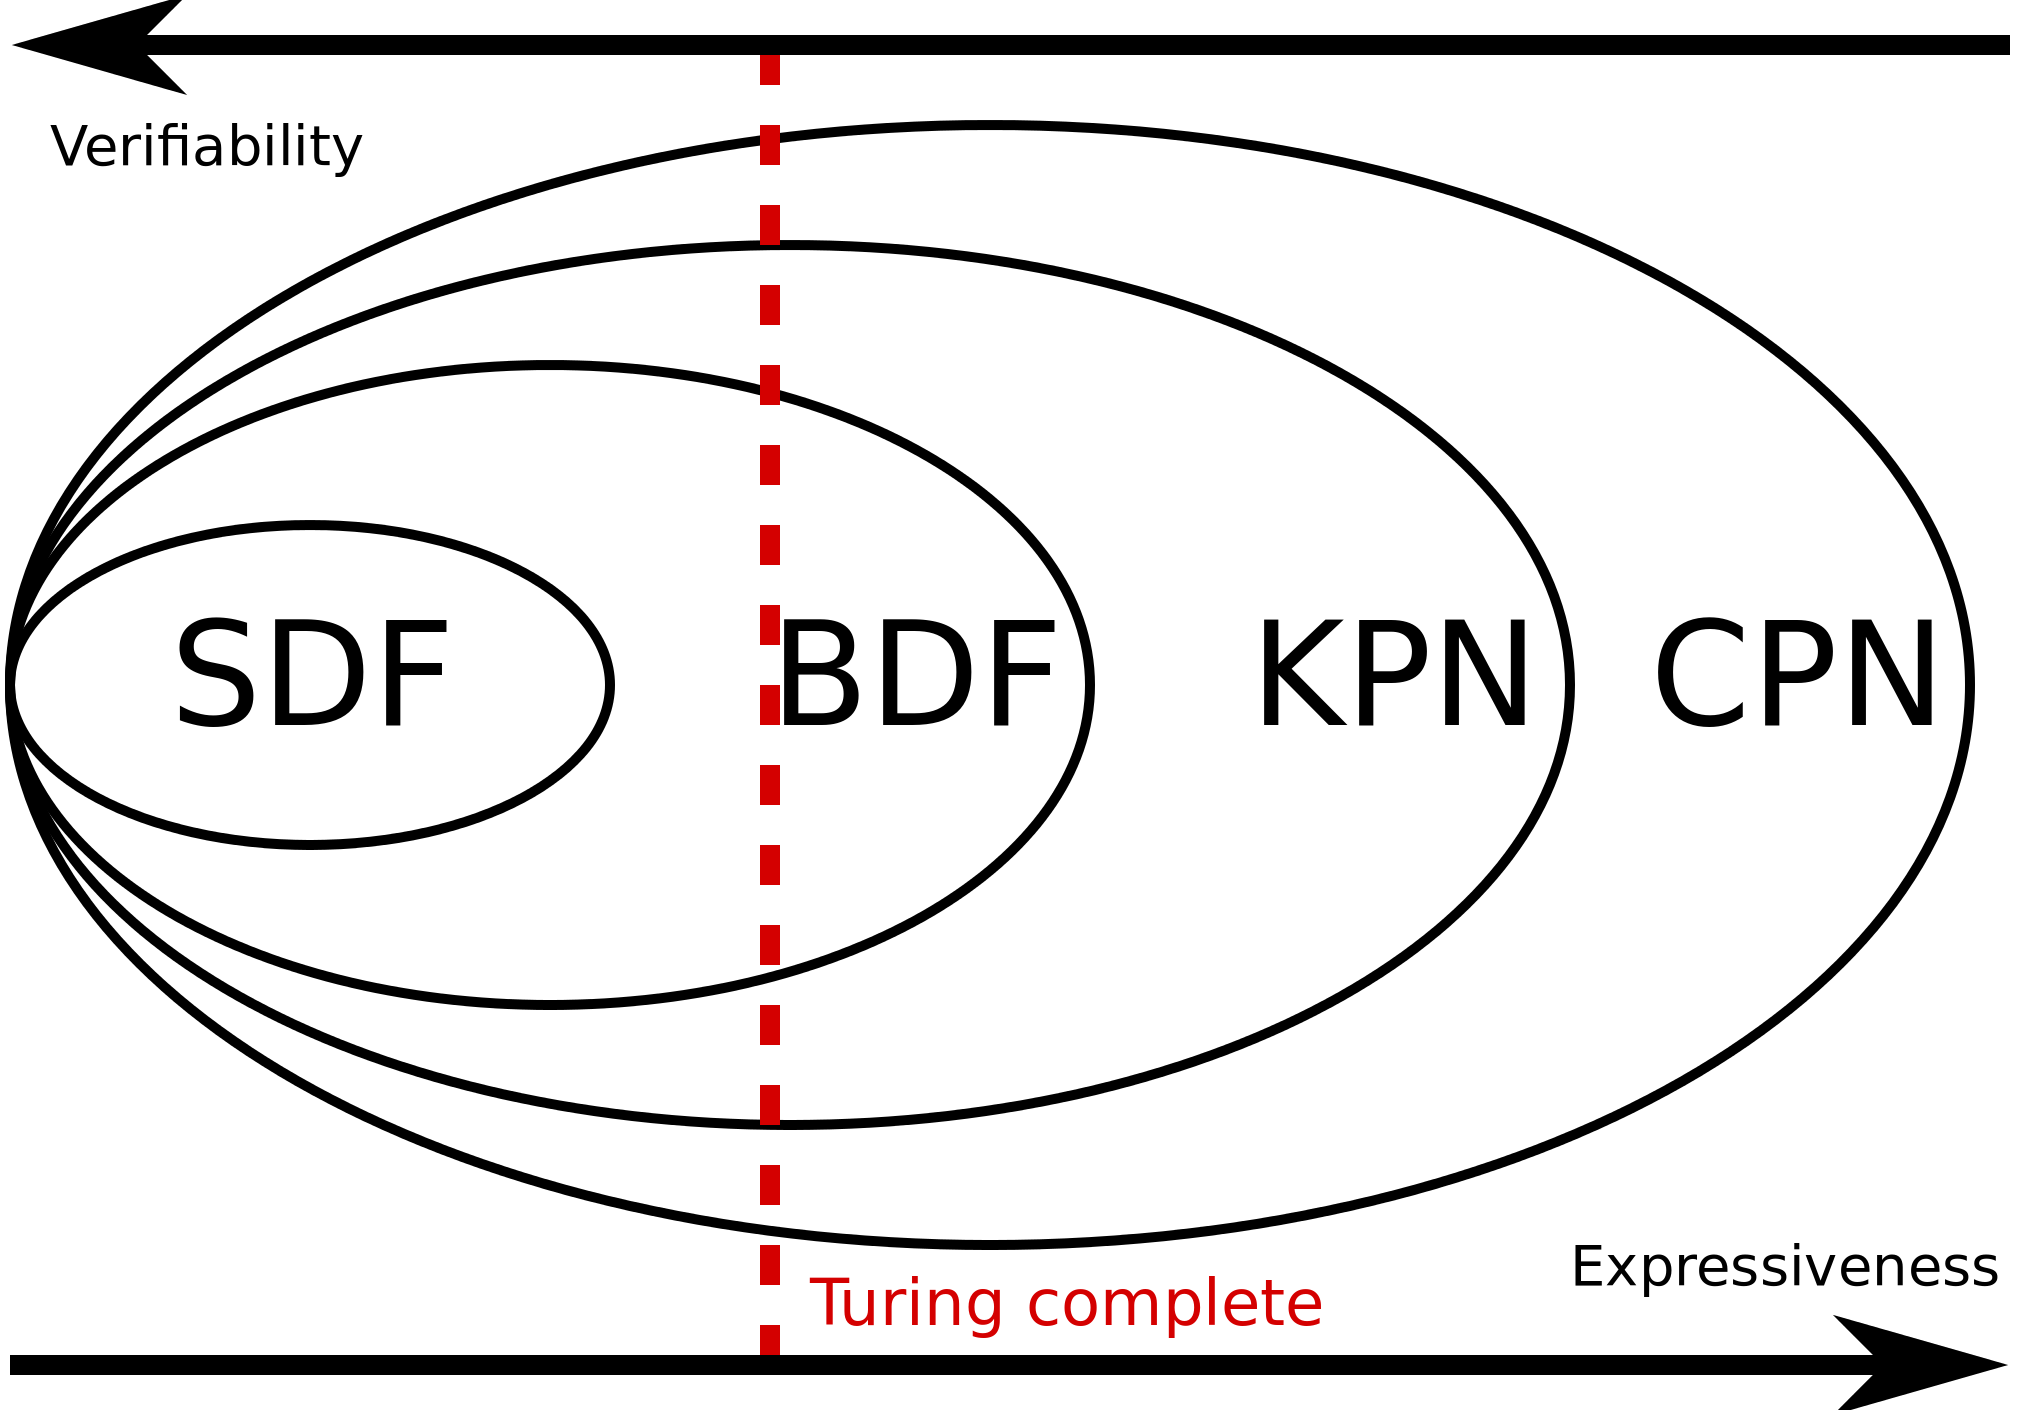
\includegraphics[width=0.5\textwidth]{pics/Verification.png}
    \caption{
        The relationship between verifiability and expressiveness for a selection of computational models.
        BDF stands for Boolean Dataflow and extends the SDF domain with data-dependent routing capabilities.
        Based on \cite{Basten}.
    }
    \label{fig:verifiability}
\end{figure}
Transaction transparency is investigated in more detail with respect to the execution semantics which specifies under what conditions a component is to be executed.
%It is closely related to the \emph{model of computation} which the framework follows.
At the one extreme there are \emph{decidable}, \emph{deterministic} models of computation
while on the other end there are \emph{undecidable}, \emph{non-deterministic} models.
To get a categorization, three well-known models have been chosen:
\begin{description}
    \item[SDF] Static Data Flow (decidable and deterministic)
    \item[KPN] Kahn Process Networks (undecidable and deterministic)
    \item[CPN] Coloured Petri Nets (undecidable and non-deterministic)
\end{description}
The execution model directly influences the possibility of verification and the expressiveness of the component networks.
The more expressive the less verifiable such a network becomes.
%Buck has found the border at which a model becomes turing-complete\cite{1993_BDF} and therefore undecidable in general.
Figure \ref{fig:verifiability} visualizes this relationship.

\subparagraph{Evaluation}
ROCK components comprise an interface consisting of inputs, outputs and parameters (properties) with data types derived from C++ types.
Furthermore, components have a life-cycle-state-machine whose state is published to the environment and can be controlled by the user.
Therefore there exist mechanisms to automatically recover from failure by monitoring the state of components. % Failure Transp.
Semantics roughly follow the KPN model; components are connected peer-to-peer through channels and are accessed by read/write functions. % Transaction Transp., Persistence Transp. because of channels
However, the user can (but shouldn't) circumvent the KPN model because emptiness of a channel can be tested.
ROCK uses message queues or CORBA for data transport dependent on the location of the interacting components. % Comm & Loc Transp.
Components can be deployed to systems with conventional processing devices capable of hosting a UNIX OS. % Resource Transp.

Behaviour Graph components (nodes) exhibit inputs and outputs with C float type.
The granularity of the atomic components is fine-grained; they are pure mathematical operators (like add, multiply etc.).
As such, their semantics follow the SDF model.
Only if all of their operands are available operations are executed.
Currently, behaviour graphs can only be executed on CPUs or $\mu$Cs and only the coordination of the components is hidden from the user.

ADE components have four types of interface links,
\begin{itemize}
    \item activation links,
    \item observation links,
    \item process control links, and
    \item component links.
\end{itemize}
Activation links are used to exchange data between components,
observation links pass state information to other components while process control links can change state,
and component links allow components to create new components.
Because of these properties the semantics of a component follow the CPN model in which non-determinism is allowed.
Communication relies on registries, servers and clients and is implemented in JAVA language as well as the components itself.
Therefore, an ADE component needs a JAVA virtual machine on top of conventional processing device (and possibly an OS).
This virtualisation and the component link mechanism provide replication transparency.
%Although it would be possible, migration transparency is not yet a property of ADE.
ADE also models computational structure of the system in form of virtual machines connected by communication links.

A GenoM3 component consists of inputs and outputs of data types defined in the Interface Description Language of CORBA.
Additionally, it defines events which are used e.g. to change state of the component.
The component behaviour is directly modeled as a Petri Net; so the semantics is of the CPN domain.
GenoM3 uses middleware templates to specify the glue code necessary for communication, distribution etc.
Therefore, all other properties strongly depend on these templates.
For example, a VHDL template could be developed which would enable GenoM to support reconfigurable hardware.
However, to the knowledge of the author such templates do not yet exist.

ROS components do not have the notion of inputs and outputs but use the concept of topics.
Topics are anonymous channels to which a ROS component can subscribe to or to which it can publish information.
As such, components are not directly coupled as in channel-based component networks.
Instead, they form a component network at run-time.
This process enables non-deterministic behavior because it is not known which component is connected to which of the others beforehand.
The semantics are therefore of the CPN domain.
As most of the previously presented frameworks, ROS also provides glue code for communication which is based on the TCP/IP stack.
The components are deployed and executed only on CPUs hosting an OS.

Although LabView is not a robotic development framework of its own, it has been used for this purpose.
The components of LabView follow the SDF semantics like those of the Behaviour Graph framework.
But the available components allow much more than purely mathematical operators; there are also components which exhibit data-dependent behaviour like loops and if-then-else structures.
LabView also provides the necessary glue code to let the components interact and it is the only framework considered here which is able to deploy them to FPGAs.
However it remains unclear if distributed operation in heterogeneous processing networks is supported by the models and the tool-chain.

\begin{table*}
	\centering
	\begin{tabular}{l|ccc}
	\hline
	Framework        & Models & Portability & Transparency\\
	\hline
	ROCK             & Sensors, Actuators & CPU \& OS & Communication, Transaction\\
	                 & & & Location, Persistence\\
	                 & & & Failure, Resource\\                 
	Behavior Graphs  &        & CPU,$\mu$C & Transaction\\
	ADE              & Sensors, Actuators & CPU \& JVM & Communication, Transaction\\
	                 & Resources, Topology & & Location, Persistence\\
	                 & & & Failure, Resource\\
	                 & & & Replication\\
	GenoM3           &        & Depends & Depends\\
	ROS              & Sensors, Actuators & CPU \& OS  & Communication, Transaction\\
	                 & & & Location, Resource\\
	LabView          & Sensors, Actuators & CPU, FPGA  & Communication, Transaction\\
	\end{tabular}
    \caption{
        Evaluation of the different frameworks.
    }
    \label{table:summary}
\end{table*}

%\paragraph{Identified Gaps and Delta}
%TODO: Verify table contents!!!!
Table~\ref{table:summary} summarizes the properties of the different frameworks.
Most frameworks exhibit a very powerful and expressive component model while only ROCK, Behaviour Graphs and LabView use a more restrictive one.
As has been stated, more expressiveness comes at the price of less verifiability.
However, the necessary tools for verification are still missing in all of the frameworks.
When it comes to critical applications like space robotics this aspect can not be neglected.

Only one framework supports different kinds of processing devices and (therefore) different programming languages.
Modern robots consist of various processing devices hosting either a CPU, a microcontroller, an FPGA or combination of them.
It is therefore essential to allow the programming of these devices and the data exchange within the framework.

To be able to distribute a given application to more than one target in a processing network the topology of it has to be modeled as well.
To the knowledge of the author only ADE considers such a model for distributing applications.
Furthermore, ADE allows dynamical redistribution during run-time which is a prerequisite to guarantee robustness against failures and load balancing.

None of the frameworks exhibits all of the properties necessary for the programming of heterogeneous and distributed robotic systems which are
\begin{itemize}
    \item distributed computation
    \item verifiability
    \item heterogeneous processing networks
    \item dynamic reprogramming (not reconfiguration via parameter updates)
\end{itemize}

% TODO: HERE IS SOMETHING MISSING!?!
%\paragraph{Related Research}
%\begin{itemize}
    %\item Partial Reconfiguration, Scrubbing
    %\item Virtualization, Middleware
    %\item HW/SW design languages (SIGNAL, Lustre)
    %\item Architecture Description Languages/Frameworks (BIP, AADL\cite{2015_Online_CMU})
    %\item Verification
%\end{itemize}
%\todo[inline]{ref to BIP}
%Some of the features needed to program a distributed, heterogeneous robotic system have been tackled within other areas of research.
%For example, the question of how to describe and model a system from both, the hardware and software perspective, is part of the development of architecture description languages/frameworks.
%Two prominent candidates in this field are the Behaviour Interaction Priority (BIP)\cite{2006_BIP} framework and the Architecture Analysis and Design Language (AADL)\cite{2015_Online_CMU}.
%Both of them allow to model the systems software by interacting component networks which is the same approach as in state-of-the-art robotic development frameworks.
%But, additionally, their component model follows a formal semantic such as to support timing analysis and verification.
%They also provide a model of the hardware components, e.g. processors, busses or memory, to which the software has to be deployed.
%Hoewever, none of them currently supports exotic targets like FPGAs.
%The TASTE toolset from ESA\cite{2012_TASTE} uses AADL in addition to other languages to support the programming of distributed, embedded real-time systems.
%Especially target architectures with devices of limited capabilties are addressed and even some basic FPGA support (by the means of accelerators) exists.
%But reconfigurable hardware is not equally treated as other, conventional devices of a robotic system.

%To be able to manage different targets to be programmed by a framework there has to be a mechanism which abstracts the details of underlying hardware.
%For conventional targets this task is mainly performed by the operating system or a virtual machine.
%On the other hand, unusual targets like FPGAs have no notion of an operating system and are programmed very differently from conventional ones.
%The HW/SW design languages like SIGNAL\cite{1991_Signal} can be used to develop software for all of these targets.
%Programs written in these languages can be easily verified because of the strict semantical models.
%The distribution of a given SIGNAL program given a simplified model of processors has been studied theoretically;
%the generated code is mainly intended for functional simulation\cite{2010_Signal}.

%The operating system BORPH\cite{2007_Borph} extends the UNIX process model to handle tasks on reconfigurable targets.
%It provides the necessary glue-code to connect the state of a hardware process to the state of a stub UNIX process.
%In contrast to the previously mentioned HW/SW design languages, BORPH handles the interconnection between individual software parts.
%But it does not provide abstraction; an expert has to design the hardware process itself before it is usable in BORPH.

%The TensorFlow\cite{2015_TensorFlow} framework can be used to define and distribute deep-learning neural networks to large-scale distributed systems.
%Although the framework makes use of graphical processing units (GPUs) the target architecture has to be homogeneous.
%All architectural entities have to have a conventional processing device and a hosting operating system to be manageable by TensorFlow.

%\paragraph{Summary}
%\begin{figure}
%    \centering
    %\includegraphics[width=0.7\textwidth]{pics/SotA_summarized.pdf}
%    \caption{
%        Schematic overview of the current state in robotic development frameworks and related areas of research.
%        The SIGNAL language and its toolset is an example of a framework supporting many heterogeneous processing devices including reconfigurable hardware devices.
%        At the other extreme, frameworks for deep-learning software like TensorFlow do not support processing devices like FPGAs
%        but support the distribution of an application to large-scale processing networks.
%    }
%    \label{fig:sota}
%\end{figure}

%Figure~\ref{fig:sota} summarizes the state-of-the-art of the robotic development frameworks embedded into the related areas of research.
%Currently, these frameworks do not model the system's processing and communication architecture,
%so the distributedness of control and the heteroegeneity of processing both are rather low.
%The SIGNAL language and its toolset are an %example of a framework supporting many %heterogeneous processing devices including %reconfigurable hardware devices.
%At the other extreme, frameworks for deep-%learning software like TensorFlow do not support %processing devices like FPGAs
%but support the distribution of an application in %large-scale processing networks.

%During the course of this activity the field of robotic development frameworks shall be extended to a domain with both, increased distributedness of the control software as well as
%better support of various, different processing devices - including reconfigurable hardware - found in modern robotic systems.

\section{Distributed Behavior Graphs}
The behavior graph formalism has been chosen as a first candidate to show the feasibility of wholistic programming of heterogeneous robots.
Because of their simplicity, the basic building blocks or atomic components are easily transferable to the FPGA-domain.
The atomic components of the behavior graphs are
\begin{itemize}
    \item N-ary reduction operations like $\Sigma,\Pi,{||.||}_{2}$
    \item Trigonometric operations ranging from $sin(x)$ to $atan2(y,x)$
    \item Other transcendental operations like $log(x)$ and $x^y$
    \item Ternary if operation (\emph{C-syntax: x = c ? a : b})
\end{itemize}
Through composition, more complex mathematical operators can be formed from the basic operations.
%In summary, behavior graphs follow the formalism presented before except for edges.
%Behavior graphs only support normal edges or binary hyper-edges respectively.
However, the formalism is not Turing-complete, because \emph{WHILE} loops or similar constructs can not be constructed.

\begin{figure}[t]
    \centering
    \subfigure[... as a CAD model]{
        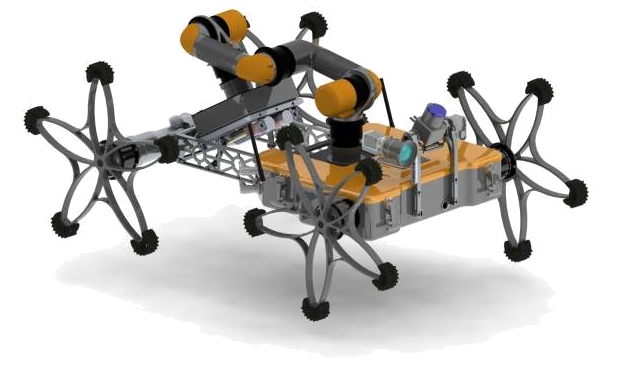
\includegraphics[width=.45\textwidth]{pics/rover.png}
    }
    \subfigure[... and a possible model of its computational infrastructure]{
        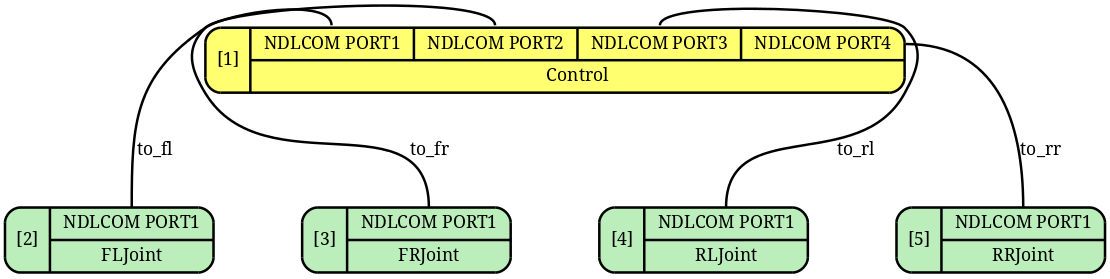
\includegraphics[width=.45\textwidth]{pics/rover-model.png}
    }
    \caption{A rover ...}
    \label{fig:rover_and_model}
\end{figure}
To model the robot hardware, a library for constructing and representing computational hardware graphs has been developed.
These hardware graphs currently support hierarchy, heterogeneity of processing elements and interfaces and point-to-point connections.
It has been designed such that other topologies, processing elements and interfaces can be added to the model easily.
Figure \ref{fig:rover_and_model} shows a rover as a CAD model and a possible computational infrastructure modelled with this library.
There is a central node \emph{Control} of type \emph{CPU} and four joints of type \emph{FPGA},
each connected to the central node via a point-to-point connection of \emph{NDLCom} interfaces (for details refer to \citep{2016_Zenzes}).

\begin{figure}[t]
    \centering
    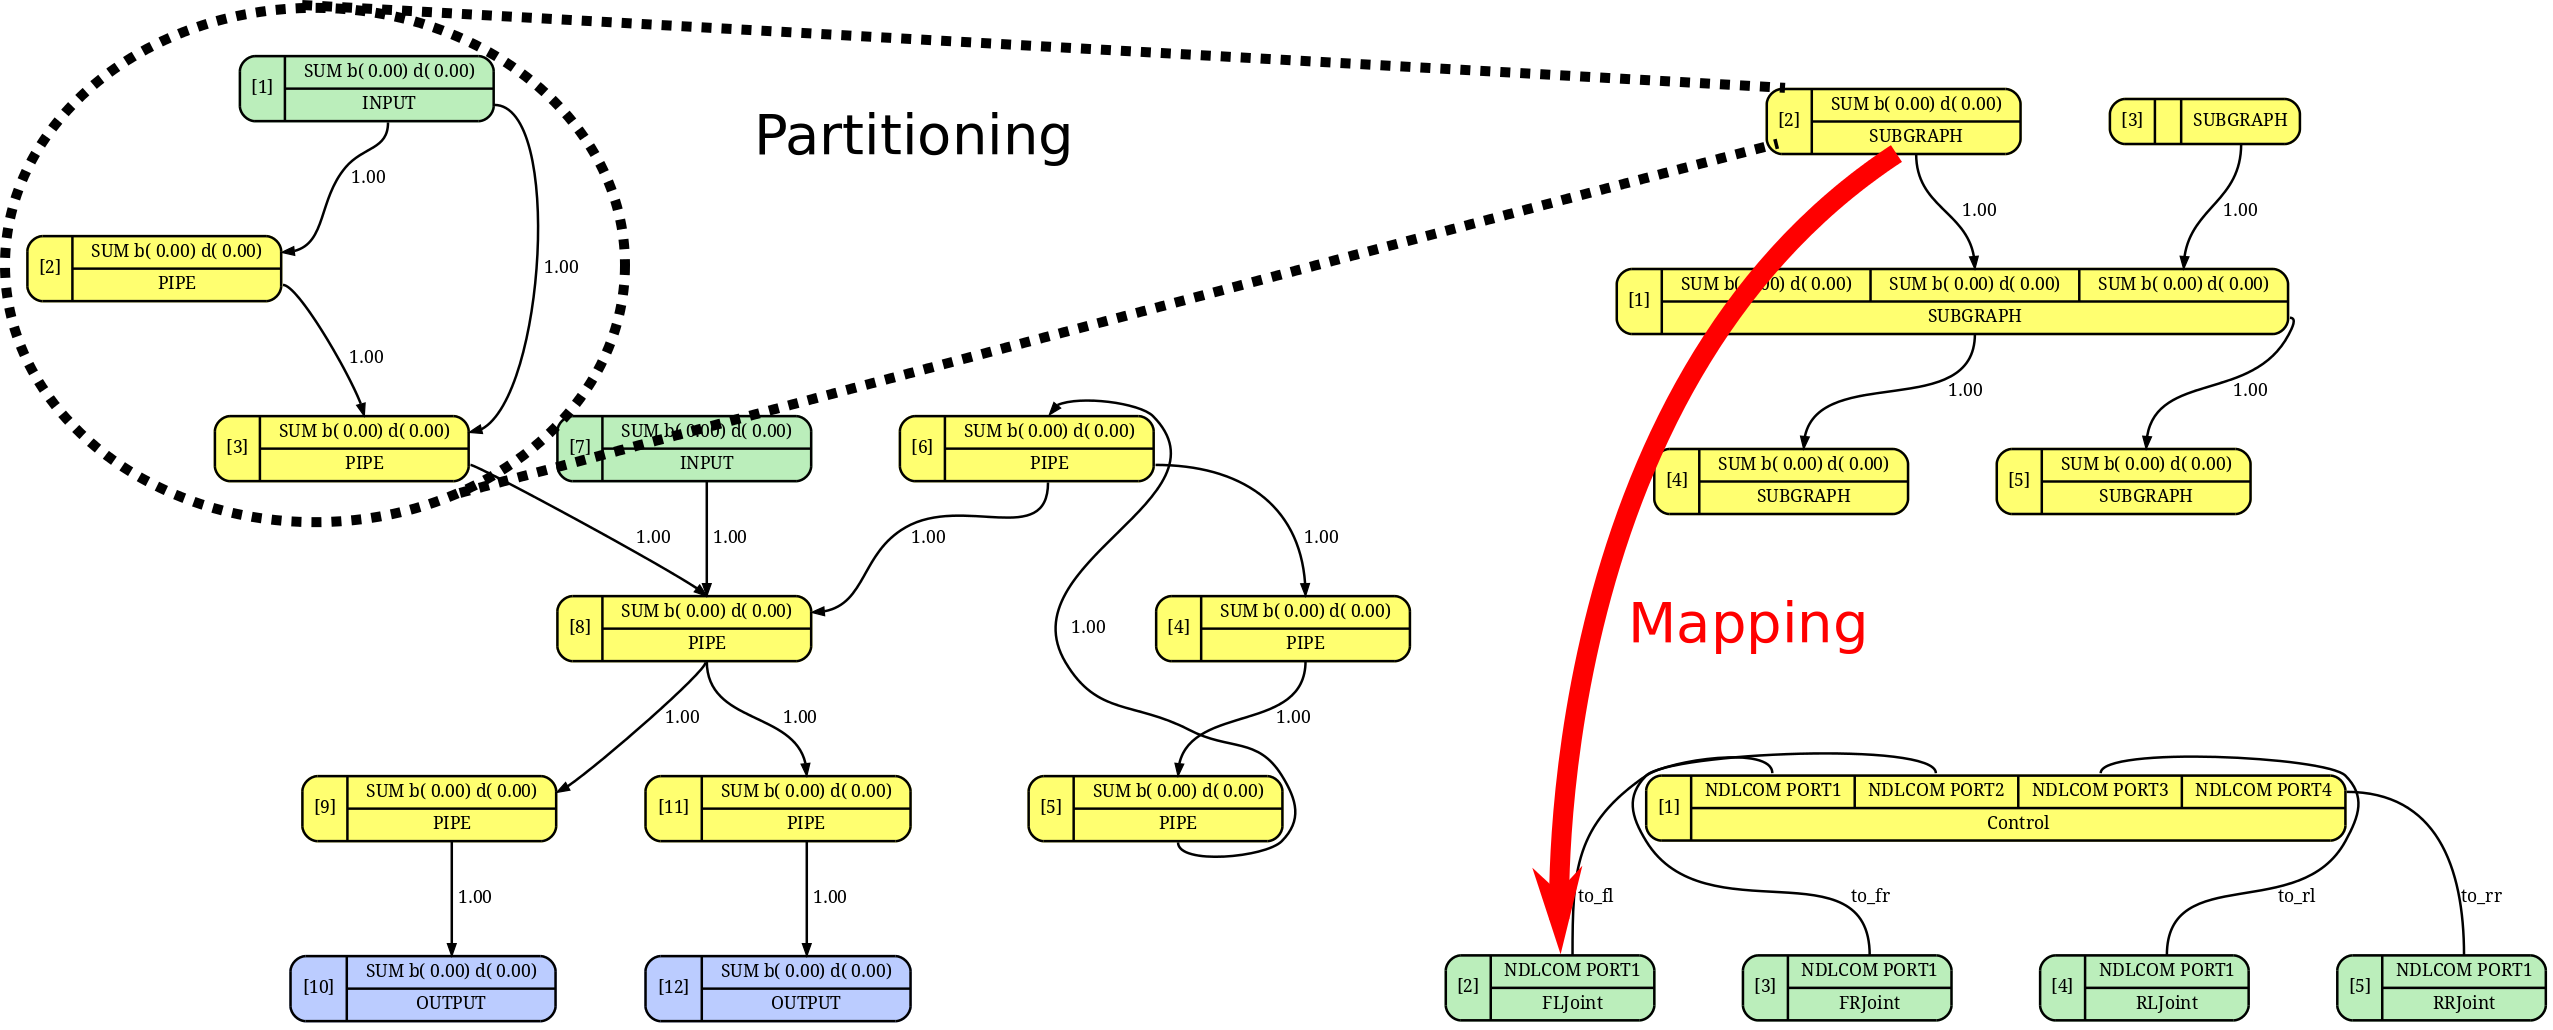
\includegraphics[width=.45\textwidth]{pics/PartAndMap.png}
    \caption{
        The behavior graph on the left is partitioned (Nodes \emph{1,2,3} to
        Node \emph{2}) to a graph of sub-graphs in the upper right.
        One of these sub-graphs has been formed for and mapped to an FPGA (Node \emph{FLJoint} in the lower right).
        Partitioning and mapping are dependent because the cost functions are target dependent in general.
    }
    \label{fig:PartAndMap}
\end{figure}
Let the left part of figure \ref{fig:PartAndMap} be a behavior graph modelling the desired control of the presented rover.
In order to exploit all computational resources and to keep latencies of control loops as short as possible,
the constituents of the control have to be assigned to the processing units such that
\begin{itemize}
    \item inputs and outputs in software match data sources and sinks in the hardware model,
    \item computational resources are shared suitably amongst the parts of the software, and
    \item communication between processing units is kept at a minimum.
\end{itemize}
These constraints are modeled by cost functions which
\begin{enumerate}
    \item have to be positive semi-definite,
    \item are target dependent in general, and
    \item must not be dependent on the order in which operations have been assigned to targets.
\end{enumerate}
Figure \ref{fig:PartAndMap} shows how a partition/sub-graph (a group of software parts) is formed and mapped to an execution target.
In this example only target-independent cost functions have been used.
One cost function increases with the number of entering or leaving edges to/from a sub-graph,
one increases with the total number of software nodes a sub-graph contains.
Partitioning and mapping is performed in two steps:
the first is to find a good initial mapping, the second is to optimize this mapping if desired.
The greedy k-way graph partitioning algorithm presented in \cite{2000_Jain} has been used to find such an initial mapping.
Afterwards optimization algorithms can be applied which check if either the re-assignment of single nodes or the permutation of whole partitions lead to global cost reduction.
% Here: Evenly distributed versus Minimal leaving/entering edges

\begin{figure}[t]
    \centering
    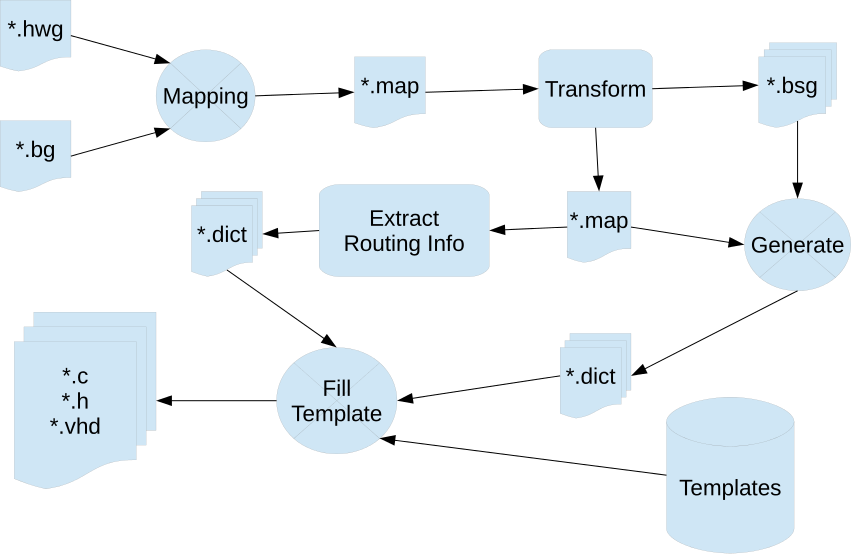
\includegraphics[width=.45\textwidth]{pics/Workflow.png}
    \caption{
        The workflow for distributing behavior graphs starts with the specification of the hardware and the desired control software and
        ends with sets of source code files ready to be deployed to the system's execution units.
    }
    \label{fig:Workflow}
\end{figure}
The complete workflow - from specification of the hardware and the software to the generation of deployments for each execution unit - is shown in figure \ref{fig:Workflow}.
According to this specification, a partitioning and mapping of the behavior graph to the execution units of the system is generated.
Each partition (stored in a \emph{*.bsg} file) is then passed to a generator which produces either \emph{C} code or \emph{VHDL} code.
This code and the routing information is used to fill source code templates which are then compiled or synthesized respectively.

These templates cover the instantiation of the behavior graph itself (most inner layer),
the separation of internal and external data sources,
the de-serialization of incoming data packets and the serialization of outgoing packets,
the triggering of the execution/evaluation of the graph (middle layer),
the setup of all external interfaces according to the hardware model,
the initialisation of the routing layer, and
the reception/transmission of behavior graph data packets.

\section{Preliminary Results}
\begin{figure}
%\begin{tikzpicture}
%    \node[align=center] (phaser) at (0,1.25) {
%        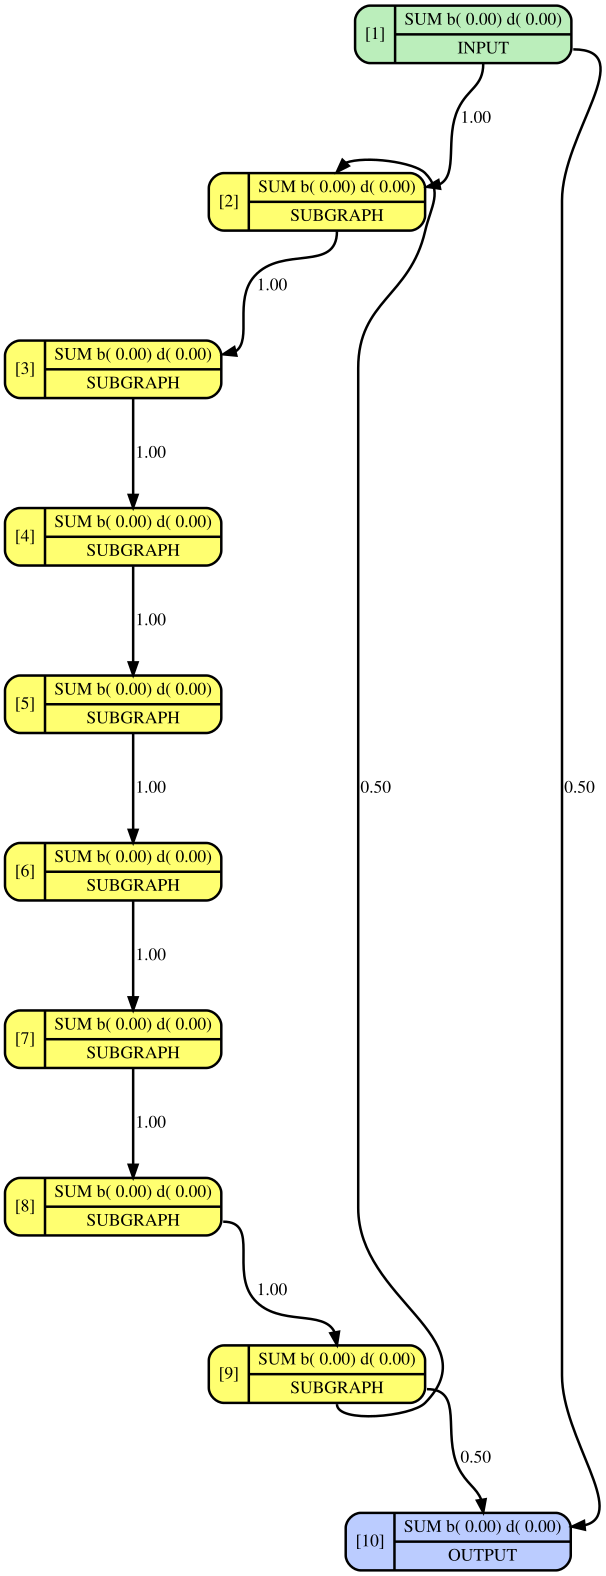
\includegraphics[width=0.25\textwidth]{pics/phaser.png}
%    };
%    \node[align=center] (allpass) at (4,5) {
%        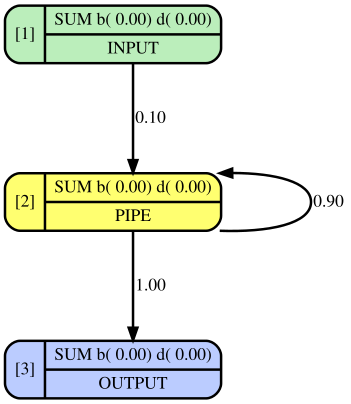
\includegraphics[width=0.15\textwidth]{pics/lowpass.png}
%    };
%    \node[align=center] (lowpass) at (4,1.75) {
%        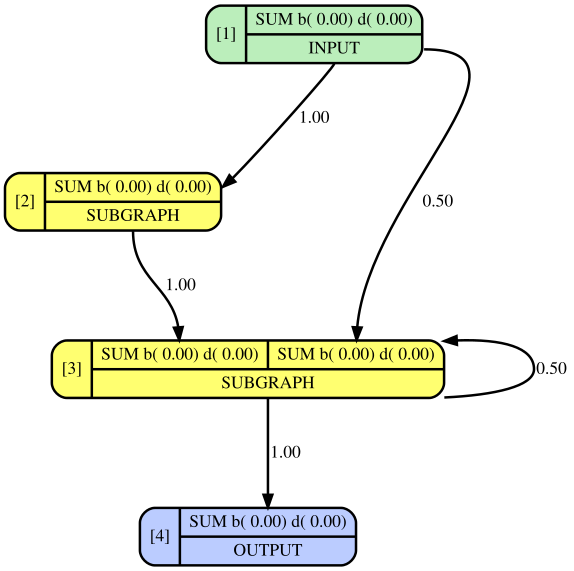
\includegraphics[width=0.225\textwidth]{pics/allpass.png}
%    };
%    \node[align=center] (opamp) at (4,-2) {
%        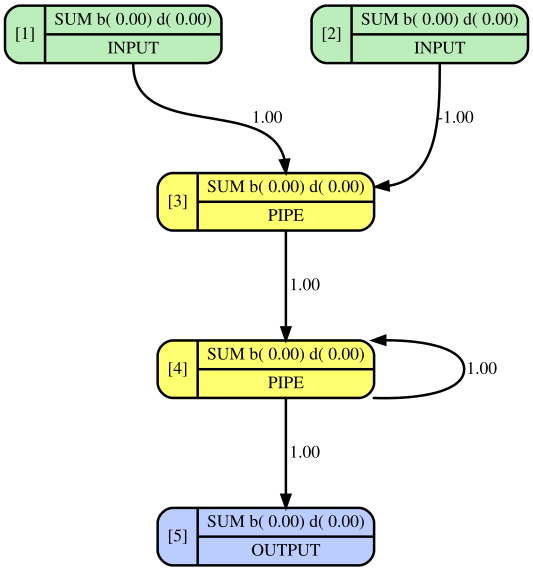
\includegraphics[width=0.225\textwidth]{pics/opamp.png}
%    };
%    \draw[-, very thick, red] (-1,3.5) -- (5,6);
%    \draw[-, very thick, red] (-1,3.5) -- (5,0);
%    \draw[-, very thick, red] (6,5) -- (5,8);
%    \draw[-, very thick, red] (6,5) -- (12,8);
%    \draw[-, very thick, red] (8,2) -- (5,-2);
%    \draw[-, very thick, red] (8,2) -- (12,-2);
%\end{tikzpicture}
	\centering
	\subfigure[Behavior graph of a phaser ...]{
		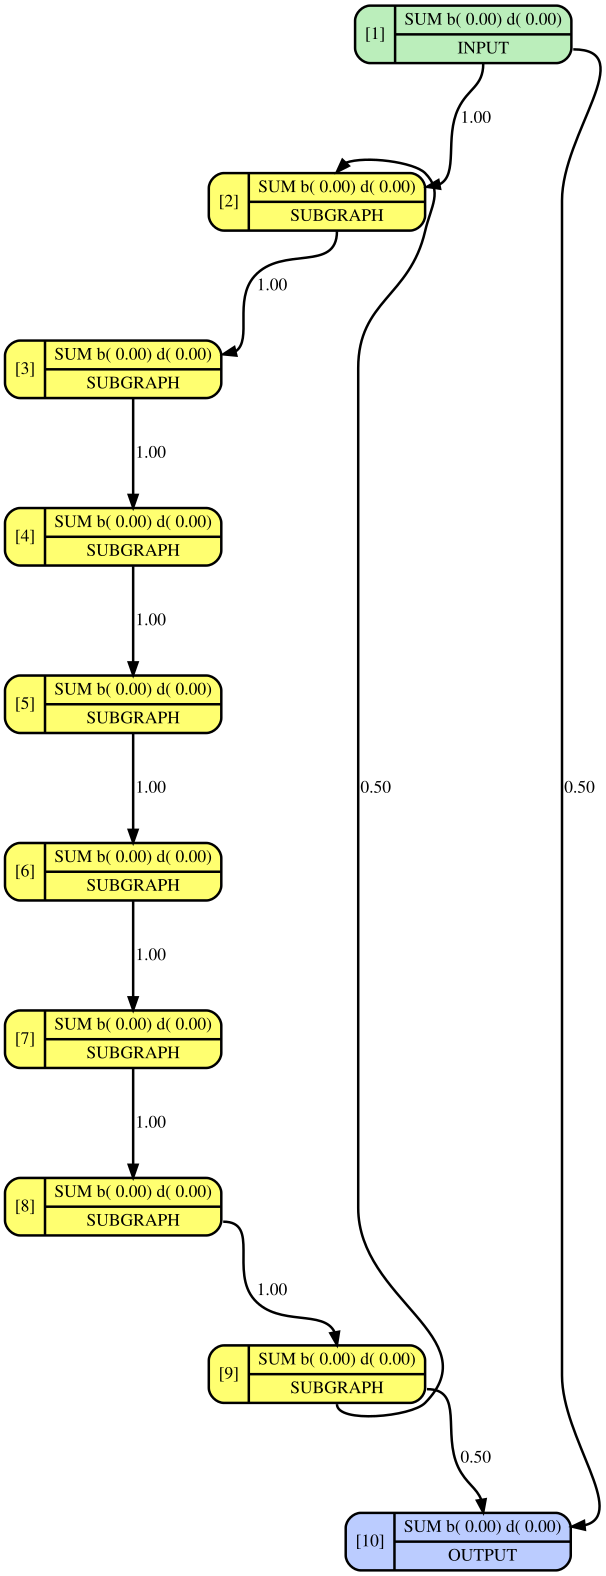
\includegraphics[width=0.2\textwidth]{pics/phaser.png}
	}
	\subfigure[... whose subgraphs are allpass filters.]{
		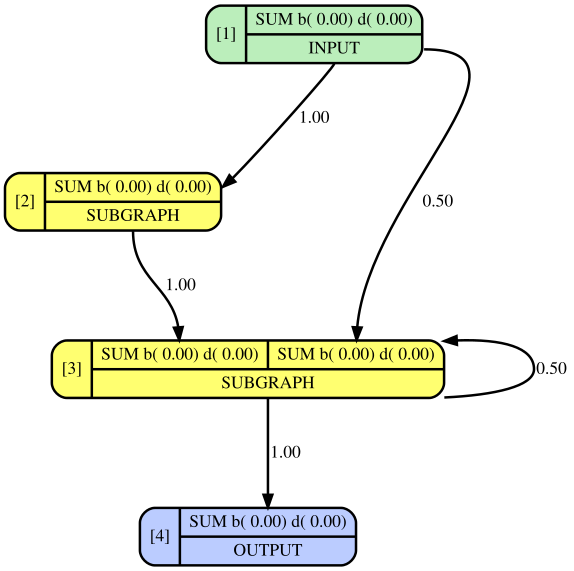
\includegraphics[width=0.2\textwidth]{pics/allpass.png}
	}
	\caption{Overview of the behavior graph used for testing.}
	\label{fig:c3po_details}
\end{figure}

\begin{figure}
\begin{tikzpicture}
    \node[align=center] (spine) at (-2,0) {
    	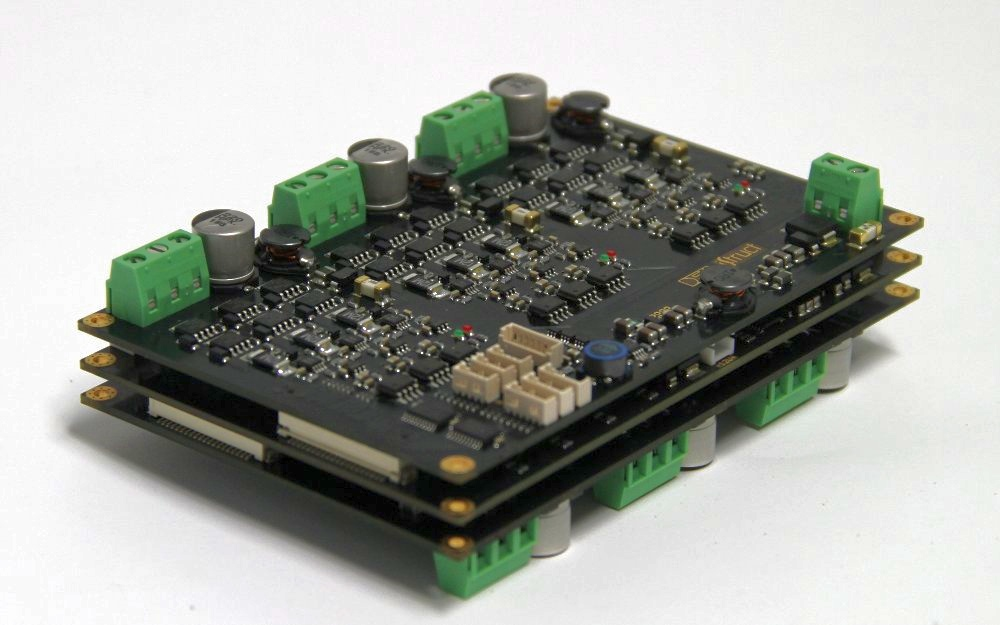
\includegraphics[width=0.2\textwidth]{pics/SpineBoard.jpg}
    };
    \node[align=center] (mdaq2) at (-2,-2.5) {
    	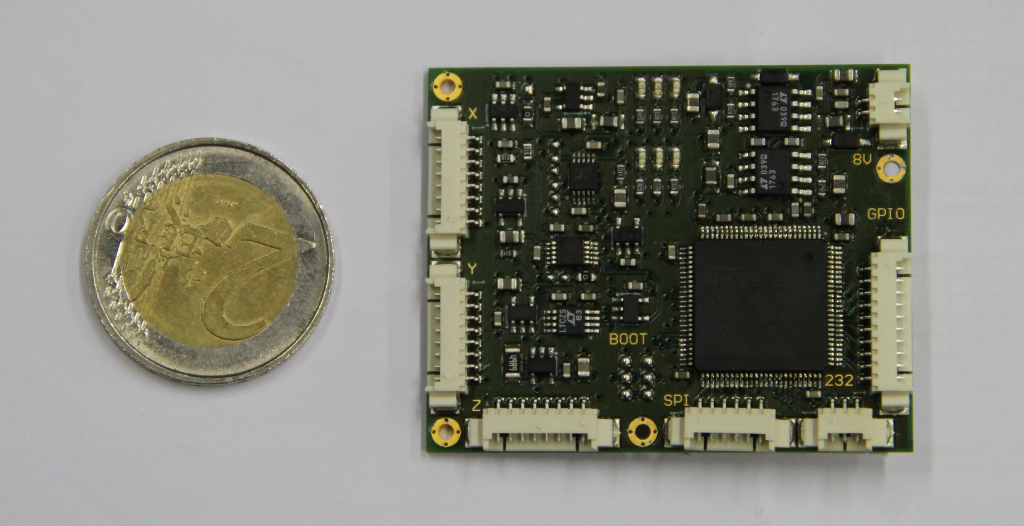
\includegraphics[width=0.2\textwidth]{pics/MDAQ2.png}
    };
    \node[align=center] (graph) at (2,-1.25) {
    	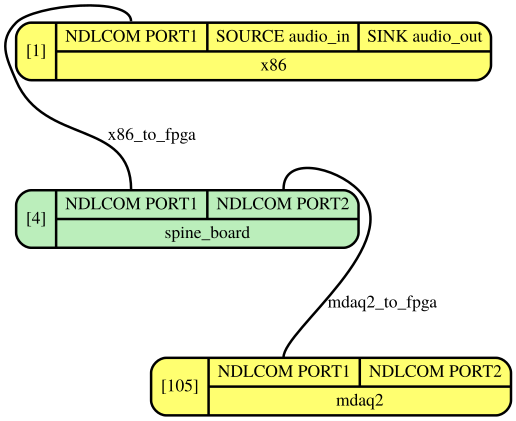
\includegraphics[width=0.25\textwidth]{pics/demo.png}
    };
\end{tikzpicture}
\caption{
The hardware setup for the preliminary tests
consisting of a standard x86, an Xilinx Spartan6 based and an ARM7 based PCB connected in series.
}
\label{fig:prelim_hw_arch}
\end{figure}

The first experiments have been performed using a conventional x86-based personal computer,
a Xilinx Spartan6 based and a ARM7 based printed circuit board (PCB) which have been interconnected in a chain.
Figure \ref{fig:prelim_hw_arch} shows photographs of the PCBs and the device interconnection.
The edges denote communication links for data exchange via the NDLCom protocol which has been developed by DFKI
and is used in various robotic systems.
%More details on the used protocol can be found in \cite{2016_Zenzes}.

The software which has been used for testing is the behavior graph shown on the left of figure \ref{fig:c3po_details}.
It resembles an audio processing network which implements the famous phaser effect used by C3PO in the Star Wars movies.
It mainly consists of an eight stage allpass filter network with feedback.
The inner workings of the allpass filters are shown on the right hand side of the figure;
the audio input is split into a lowpass (shown in the upper right) filtered and a non-filtered stream which are then
fed into an (ideal) operational amplifier (shown in the lower right).

\begin{figure}
\begin{tikzpicture}
    \node[align=center] (undistorted) at (-2,0) {
    	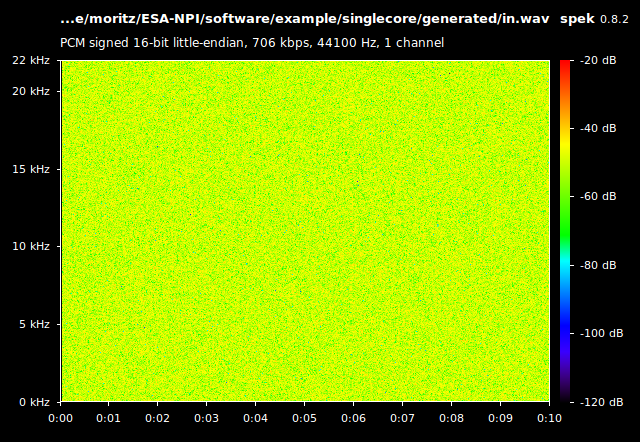
\includegraphics[width=0.225\textwidth]{pics/whitenoise_orig.png}
    };
    \node[align=center] (distorted) at (2,0) {
    	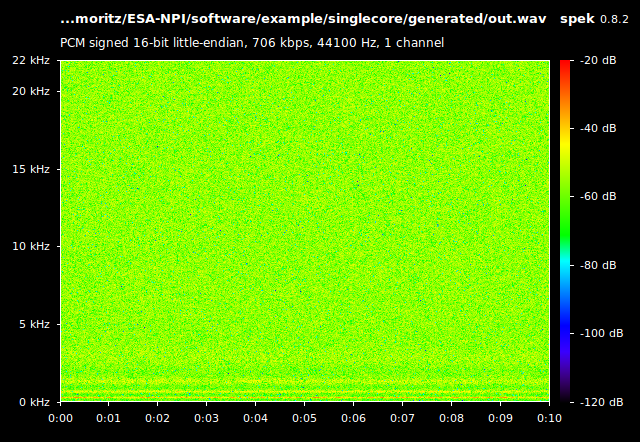
\includegraphics[width=0.225\textwidth]{pics/whitenoise_filtered.png}
    };
    \node[align=center, draw, red, very thick] (zoomed) at (2.5,0) {
    	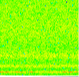
\includegraphics[width=0.075\textwidth]{pics/whitenoise_filtered_zoom.png}
    };
    %\draw[-, dashed, red, very thick] (0,-1.7) -- (2,-1.7);
    \draw[-, dashed, red, very thick] (0.5,-0.75) -- (1.75,0.5);
    %\draw[-, dashed, red, very thick] (0,-2.1) -- (2,-2.1);
    \draw[-, dashed, red, very thick] (0.5,-1.1) -- (1.75,-0.5);
    \draw[-, dashed, red, very thick] (0.85,-1.1) -- (3,-0.65);
\end{tikzpicture}
\caption{
The spectra of the original white noise test signal (left) and the filtered test signal (right) over time.
In the filtered signal the peaks of the transfer function can be observed for signals below 5 kHz.
}
\label{fig:prelim_results}
\end{figure}

To find out about the transfer function of the network,
a signal with a uniform distribution of frequencies or white noise respectively is streamed into it.
The filtered signal should exhibit three sharp peaks and four notches in the spectrum.
Figure \ref{fig:prelim_results} is showing, that this can be observed in the frequency range below 5 kHz.
The left figure represents the spectrum of the undistorted white noise, while the right shows the filtered signal.
The peaks have been highlighted by red lines.

\section{Outlook}
% Refer to hypergraphs, ontologies etc.
% Open issues
% - fixed instruction/component set
% - no non-determinism (at least controlled non-determinism)
% - tool-chain does not reuse previously generated stuff
% - model domains are separate, there is no fundamental model
%   hosting both
% - model domains are fixed and not easily extendable
% - No mechanism to ensure correctness or to reason about it
The distributed behavior graph framework is able to generate and distribute networks of simple, fixed mathematical operators to a network of distributed processing units.
But to be useful for general purpose application aside from signal processing the instruction set itself should be adaptable either to store already generated sub-graphs, to allow more powerful, possibly non-deterministic operators or multiple implementations for the same algorithm/instruction.

The behavior graph model and the hardware model are based on graphs but there is no underlying model (yet) which allows both modelling domains to be easily incorporated into higher-level domains (such as the mapping domain).
A fundamental model would also enable the possibility of extending the different views on a robotic system by e.g. adding models of the electrical wiring or the kinematic structure.

It is planned to utilize ontologies to serve as the basis for the different domains.
This will also enable the framework to ensure certain constraints between e.g. the interconnection of devices or software components.

\bibliographystyle{aa}
\bibliography{References}

\end{document}
